%===================================================================================
% JORNADA CIENTÍFICA ESTUDIANTIL - MATCOM, UH
%===================================================================================
% Esta plantilla ha sido diseñada para ser usada en los artículos de la
% Jornada Científica Estudiantil de MatCom.
%
% Por favor, siga las instrucciones de esta plantilla y rellene en las secciones
% correspondientes.
%
% NOTA: Necesitará el archivo 'jcematcom.sty' en la misma carpeta donde esté este
%       archivo para poder utilizar esta plantila.
%===================================================================================



%===================================================================================
% PREÁMBULO
%-----------------------------------------------------------------------------------
\documentclass[a4paper,10pt,twocolumn]{article}

%===================================================================================
% Paquetes
%-----------------------------------------------------------------------------------
\usepackage{amsmath}
\usepackage{amsfonts}
\usepackage{amssymb}
\usepackage{jcematcom}
\usepackage[utf8]{inputenc}
\usepackage{listings}
\usepackage[pdftex]{hyperref}
\usepackage{caption}
\usepackage{subcaption}

\usepackage{listings}
\usepackage{xcolor}

%-----------------------------------------------------------------------------------
% Configuración
%-----------------------------------------------------------------------------------
\hypersetup{colorlinks,%
	    citecolor=black,%
	    filecolor=black,%
	    linkcolor=black,%
	    urlcolor=blue}


\colorlet{punct}{red!60!black}
\definecolor{background}{HTML}{EEEEEE}
\definecolor{delim}{RGB}{20,105,176}
\colorlet{numb}{magenta!60!black}

\lstdefinelanguage{json}{
	basicstyle=\normalfont\ttfamily,
	numbers=left,
	numberstyle=\scriptsize,
	stepnumber=1,
	numbersep=8pt,
	showstringspaces=false,
	breaklines=true,
	frame=lines,
	backgroundcolor=\color{background},
	literate=
		*{0}{{{\color{numb}0}}}{1}
		{1}{{{\color{numb}1}}}{1}
		{2}{{{\color{numb}2}}}{1}
		{3}{{{\color{numb}3}}}{1}
		{4}{{{\color{numb}4}}}{1}
		{5}{{{\color{numb}5}}}{1}
		{6}{{{\color{numb}6}}}{1}
		{7}{{{\color{numb}7}}}{1}
		{8}{{{\color{numb}8}}}{1}
		{9}{{{\color{numb}9}}}{1}
		{:}{{{\color{punct}{:}}}}{1}
		{,}{{{\color{punct}{,}}}}{1}
		{\{}{{{\color{delim}{\{}}}}{1}
		{\}}{{{\color{delim}{\}}}}}{1}
		{[}{{{\color{delim}{[}}}}{1}
		{]}{{{\color{delim}{]}}}}{1},
}

%===================================================================================



%===================================================================================
% Presentacion
%-----------------------------------------------------------------------------------
% Título
%-----------------------------------------------------------------------------------
\title{Proyecto de Modelos de Matemática Aplicada. \\Construcción y graficación de grafos causales}

%-----------------------------------------------------------------------------------
% Autores
%-----------------------------------------------------------------------------------
\author{\\
\name Dennis Fiallo Muñoz \email \href{mailto: dennis.fiallo@estudiantes.matcom.uh.cu}{dennis.fiallo@estudiantes.matcom.uh.cu}
	\\ \addr Grupo C-311 \AND
\name Lauren O. Guerra Herández \email \href{mailto:lauren.guerra@estudiantes.matcom.uh.cu}{lauren.guerra@estudiantes.matcom.uh.cu}
  \\ \addr Grupo C-312}

%-----------------------------------------------------------------------------------
% Tutores
%-----------------------------------------------------------------------------------
\tutors{\\
Dr. Ferando Rodríguez Flores \emph{MatCom} \\
Lic. Ania , \emph{MatCom}}

%-----------------------------------------------------------------------------------
% Headings
%-----------------------------------------------------------------------------------
\jcematcomheading{\the\year}{1-\pageref{end}}{D. Fiallo, L. Guerra}

%-----------------------------------------------------------------------------------
\ShortHeadings{Ejemplo JCE}{Autores}
%===================================================================================



%===================================================================================
% DOCUMENTO
%-----------------------------------------------------------------------------------
\begin{document}

%-----------------------------------------------------------------------------------
% NO BORRAR ESTA LINEA!
%-----------------------------------------------------------------------------------
\twocolumn[
%-----------------------------------------------------------------------------------

\maketitle

%===================================================================================
% Resumen y Abstract
%-----------------------------------------------------------------------------------
\selectlanguage{spanish} % Para producir el documento en Español

%-----------------------------------------------------------------------------------
% Resumen en Español
%-----------------------------------------------------------------------------------
\begin{abstract}

El presente proyecto se encarga de resolver un problema práctico para matemáticos que realizan estudios sobre el cerebro humano. Es una herramienta creada específicamente para facilitar la visualización de modelaciones del cerebro y sus conexiones a partir de grafos causales. Para esto a partir de modelaciones en matrices previamente realizadas se contruyen grafos con ayuda de la librería gravis y se visualizan cómodamente en una interfaz visual web.\\
Para más información sobre la interfaz visual del proyecto ver el manual de usuario en: $\href{https://github.com/dionisio35/graph_plotting/tree/main/user manual}{https://github.com/dionisio35/graph_plotting/tree/main/user manual}$\\
Para acceder al código fuente del proyecto ir a: $\href{https://github.com/dionisio35/graph_plotting}{https://github.com/dionisio35/graph_plotting}$


\end{abstract}

%-----------------------------------------------------------------------------------
% English Abstract
%-----------------------------------------------------------------------------------
\vspace{0.5cm}

\begin{enabstract}

This project is responsible for solving a practical problem for mathematicians who carry out studies on the human brain. It is a tool created specifically to facilitate the visualization of models of the brain and its connections from causal graphs. For this, based on matrix modeling previously carried out, graphs are built with the help of the gravis library and are conveniently displayed in a visual web interface.
\\
For more information about the visual interface of the project, see the user manual at: $\href{https://github.com/dionisio35/graph_plotting/tree/main/user manual}{https://github.com/dionisio35/graph_plotting/tree/main/user manual}$\\
To access the source code of the project go to:  $\href{https://github.com/dionisio35/graph_plotting}{https://github.com/dionisio35/graph_plotting}$
\end{enabstract}

%-----------------------------------------------------------------------------------
% Palabras clave
%-----------------------------------------------------------------------------------
\begin{keywords}
	grafos causales,
	librerías,
	módulos,
	conexiones causales,
	conexiones contemporáneas
	python
\end{keywords}

%-----------------------------------------------------------------------------------
% Temas
%-----------------------------------------------------------------------------------
%\begin{topics}
%	Tema, Subtema.
%\end{topics}


%-----------------------------------------------------------------------------------
% NO BORRAR ESTAS LINEAS!
%-----------------------------------------------------------------------------------
\vspace{1.8cm}
]
%-----------------------------------------------------------------------------------


%===================================================================================

%===================================================================================
% Introducción
%-----------------------------------------------------------------------------------
\section*{Introducción}\label{sec:intro}
%-----------------------------------------------------------------------------------

Se necesita para investigaciones en el Centro de Neurociencias de Cuba una aplicación que ayude a los investigadore a representar en forma de grafo las de conexiones causales y contemporánea que ocurren en el cerebro humano para esto nos proponemos hacer un programa al cual se le pasen dos tensores de conectividad y una lista con los nombres de los nodos y con estos datos construir un grafo que admita las 360 conexiones necesitadas y además se vea de la mejor manera posible para apoyar su estudio y análisis.\\

El proceso de contrucción de grafo causales se realiza a partir de dos tensores de 360x360xlags, siendo uno binario indicando si hubo conexión o no, y otro de pesos indicando la fuerza de las conexiones. Estos se construyen de la siguiente manera:

\begin{description}


\item	Conexiones contemporáneas: Se representan con una línea recta. Se toma el lag 0(único lag simétrico) y donde aparezca 1 significa que hay conexión entre los nodos (i, j), mientras que el color de la conexión que se traza viene dado por el valor de la matriz de peso en la posición (i, j).\\

\item	Lagged connections o causalidad: Se representan con flechas. Para el resto de lags se busca igualmente si hay un 1 en el tensor binario de 
lag$\neq $0 y se construye una flecha del nodo i al j con la intensidad dada por el promedio de los valores de la matriz de pesos en los lags donde hubo conexión, además de especificar los lags con conexión.\\

\end{description}

\begin{figure}[h!]%
\center
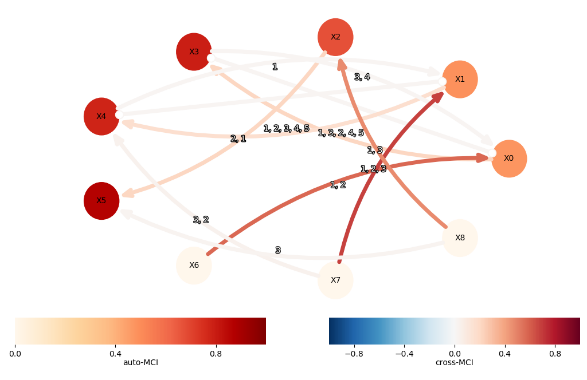
\includegraphics[scale=0.95]{example1.png}
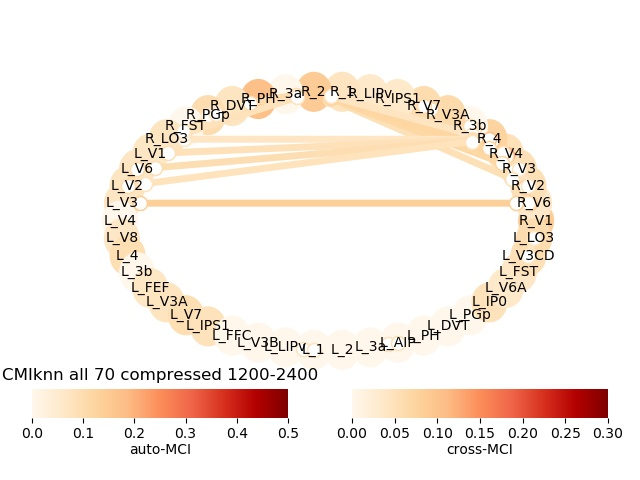
\includegraphics[scale=0.45]{example.png}
\caption{Ejemplo de graficación de grafos causales que se pueden ver con precisión}
\end{figure}

\newpage


Las aplicaciones con las que cuenta el usuario al pasarle un gráfico de más de 180 series de tiempo(en la práctica se necesitan 360), el programa pone 180 nodos sobre una circunferencia y los restantes los sobrepone a estos en la misma circunferencia, haciendo que no sea posible ver las conexiones.\\


\begin{figure}[h!]%
\center
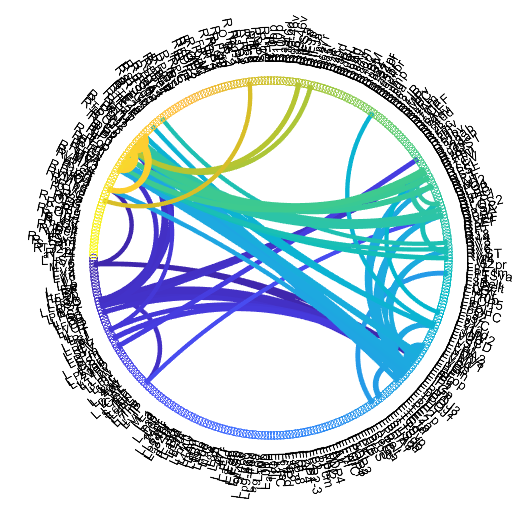
\includegraphics[scale=0.3]{example2.png}
\caption{Ejemplo de graficación en que los nodos se superponen y no se pueden observar los resultados}
\end{figure}
 
 
Por esto nuestro objetivo es hacer un programa al cual se le pasen dos tensores de conectividad y una lista con los nombres de los nodos y construir un grafo como se explicó anteriormente que admita las 360 necesarias y en general la cantidad de conexiones que se necesiten representar en cada caso y se puedan ver correctamente los nodo, las conexiones y la fuerza de estas. \\

También otro problema que presenta el usuario es que guarda cada uno de los pares de tensores que se utilizan para la contrucción de los grafos en formato matlab, donde cada archivo .mat que contiene un par de tensores ocupa un espacio de más de 3.0 mb, por lo cual al tener cientos de archivos de este tipo para su investigación ocupan un espacio considerable, por esto además nos propusimos que una vez conformado el grafo, sea guardado en un archivo que pese mucho menos y luego este pueda ser cargado desde nuestra misma aplicación. 

\section*{Primeras ideas}

Al comienzo de la realización de este proyecto se tenía en mente la implementación de métodos para dibujar grafos que lograran una buena ditribución de nodos y aristas en el espacio bidimensional utilizando los conocimientos adquiridos en asignaturas como Matemática Discreta II, Estructura de Datos y Algoritmos II y Modelos de Optimización, esto dibujando el grafo en su forma maximal planar y luego ir añadiendo las aristas que falten por dibujarse  minimizando la cantidad de aristas que serían dibujadas cortando a las que ya estuvieran colocadas. \\

Esto tuvo grandes inconvenientes porque los grafo causales, sobre todo el de conexiones contemporáneas, están muy lejos de ser planares, tienen muchas aristas y a la hora de acomodar los nodos y dibujar las aristas que no formaban parte del grafo maximal planar tomado como base no se podían garantizar distrubuciones de nodos y aristas que dieran lugar a la correcta observación del grafo.\\

Buscando en el estado del arte no existía nada como esto, ninguna distribución que se hiciera a un grafo resultaba buena en todos los casos, para todo tipo de grafos, probamos con la librería networkx las diferentes distribuciones que esta tiene implementadas y ninguna de ellas cumplía nuestro objetivo, por lo que llegamos a la conclusión que crear un algoritmo que graficara cualquier grafo de la mejor manera poible para él es un ejercicio muy complicado por lo cual no se encontraba a nuestro alcance.\\

Por esto nos propusimos utilizar las mejores implementaciones de dibujo de grafos que estuvieran disponibles en librerías de python para poder resolver el problema del usuario y lograr su satisfacción y comodidad.\\



\section*{Solución}
El proyecto se encuentra programado en su totalidad en Python. Para la graficación de los grafos causales
se usa el módulo gravis \cite{gv}; su nombre significa \texttt{graph visualization}, visualización de grafos,
y como su nombre indica, está destinado a la creación de grafos interactivos en 2d y 3d.
Usa tecnologías como \texttt{HTML}, \texttt{CSS} y \texttt{JS} para representar los grafos, apoyándose en gran medida de
módulos como \texttt{d3.js}, \texttt{vis.js} y \texttt{three.js}( las representaciones visuales basadas en estos módulos
se presentan en el proyecto como \texttt{Graph}, \texttt{Complex Graph} y \texttt{3D Graph} respectivamente).
Para mostrar los resultados se usa en la interfáz visual se usa el módulo streamlit \cite{st}, tomando la información proporcionada por gravis como HTML.\\

Para la representación de los grafos en el proyecto se usa el mismo formato que se usa en \texttt{gravis}, gravis JSON Graph Format(\texttt{gJGF}),
el cual se define como \texttt{dict} en Python generándose como se muestra a continuación:

\begin{lstlisting}[language=json,firstnumber=1]
{
	"graph":{
		"metadata": {},
		"directed": bool,
		"nodes": {},
		"edges": []
	}	
}
\end{lstlisting}


Para la representación de los grafos se puede indicar desde el inicio las posiciones espaciales de cada nodo,
como es el caso del \texttt{3D Graph} que presentamos con con ubicaciones reales a escala de las areas estimuladas del cerebro.
Sin embargo en el resto de los casos se usan algoritmos apoyados en las físicas para representar los nodos.\\

\begin{figure}[h!]%
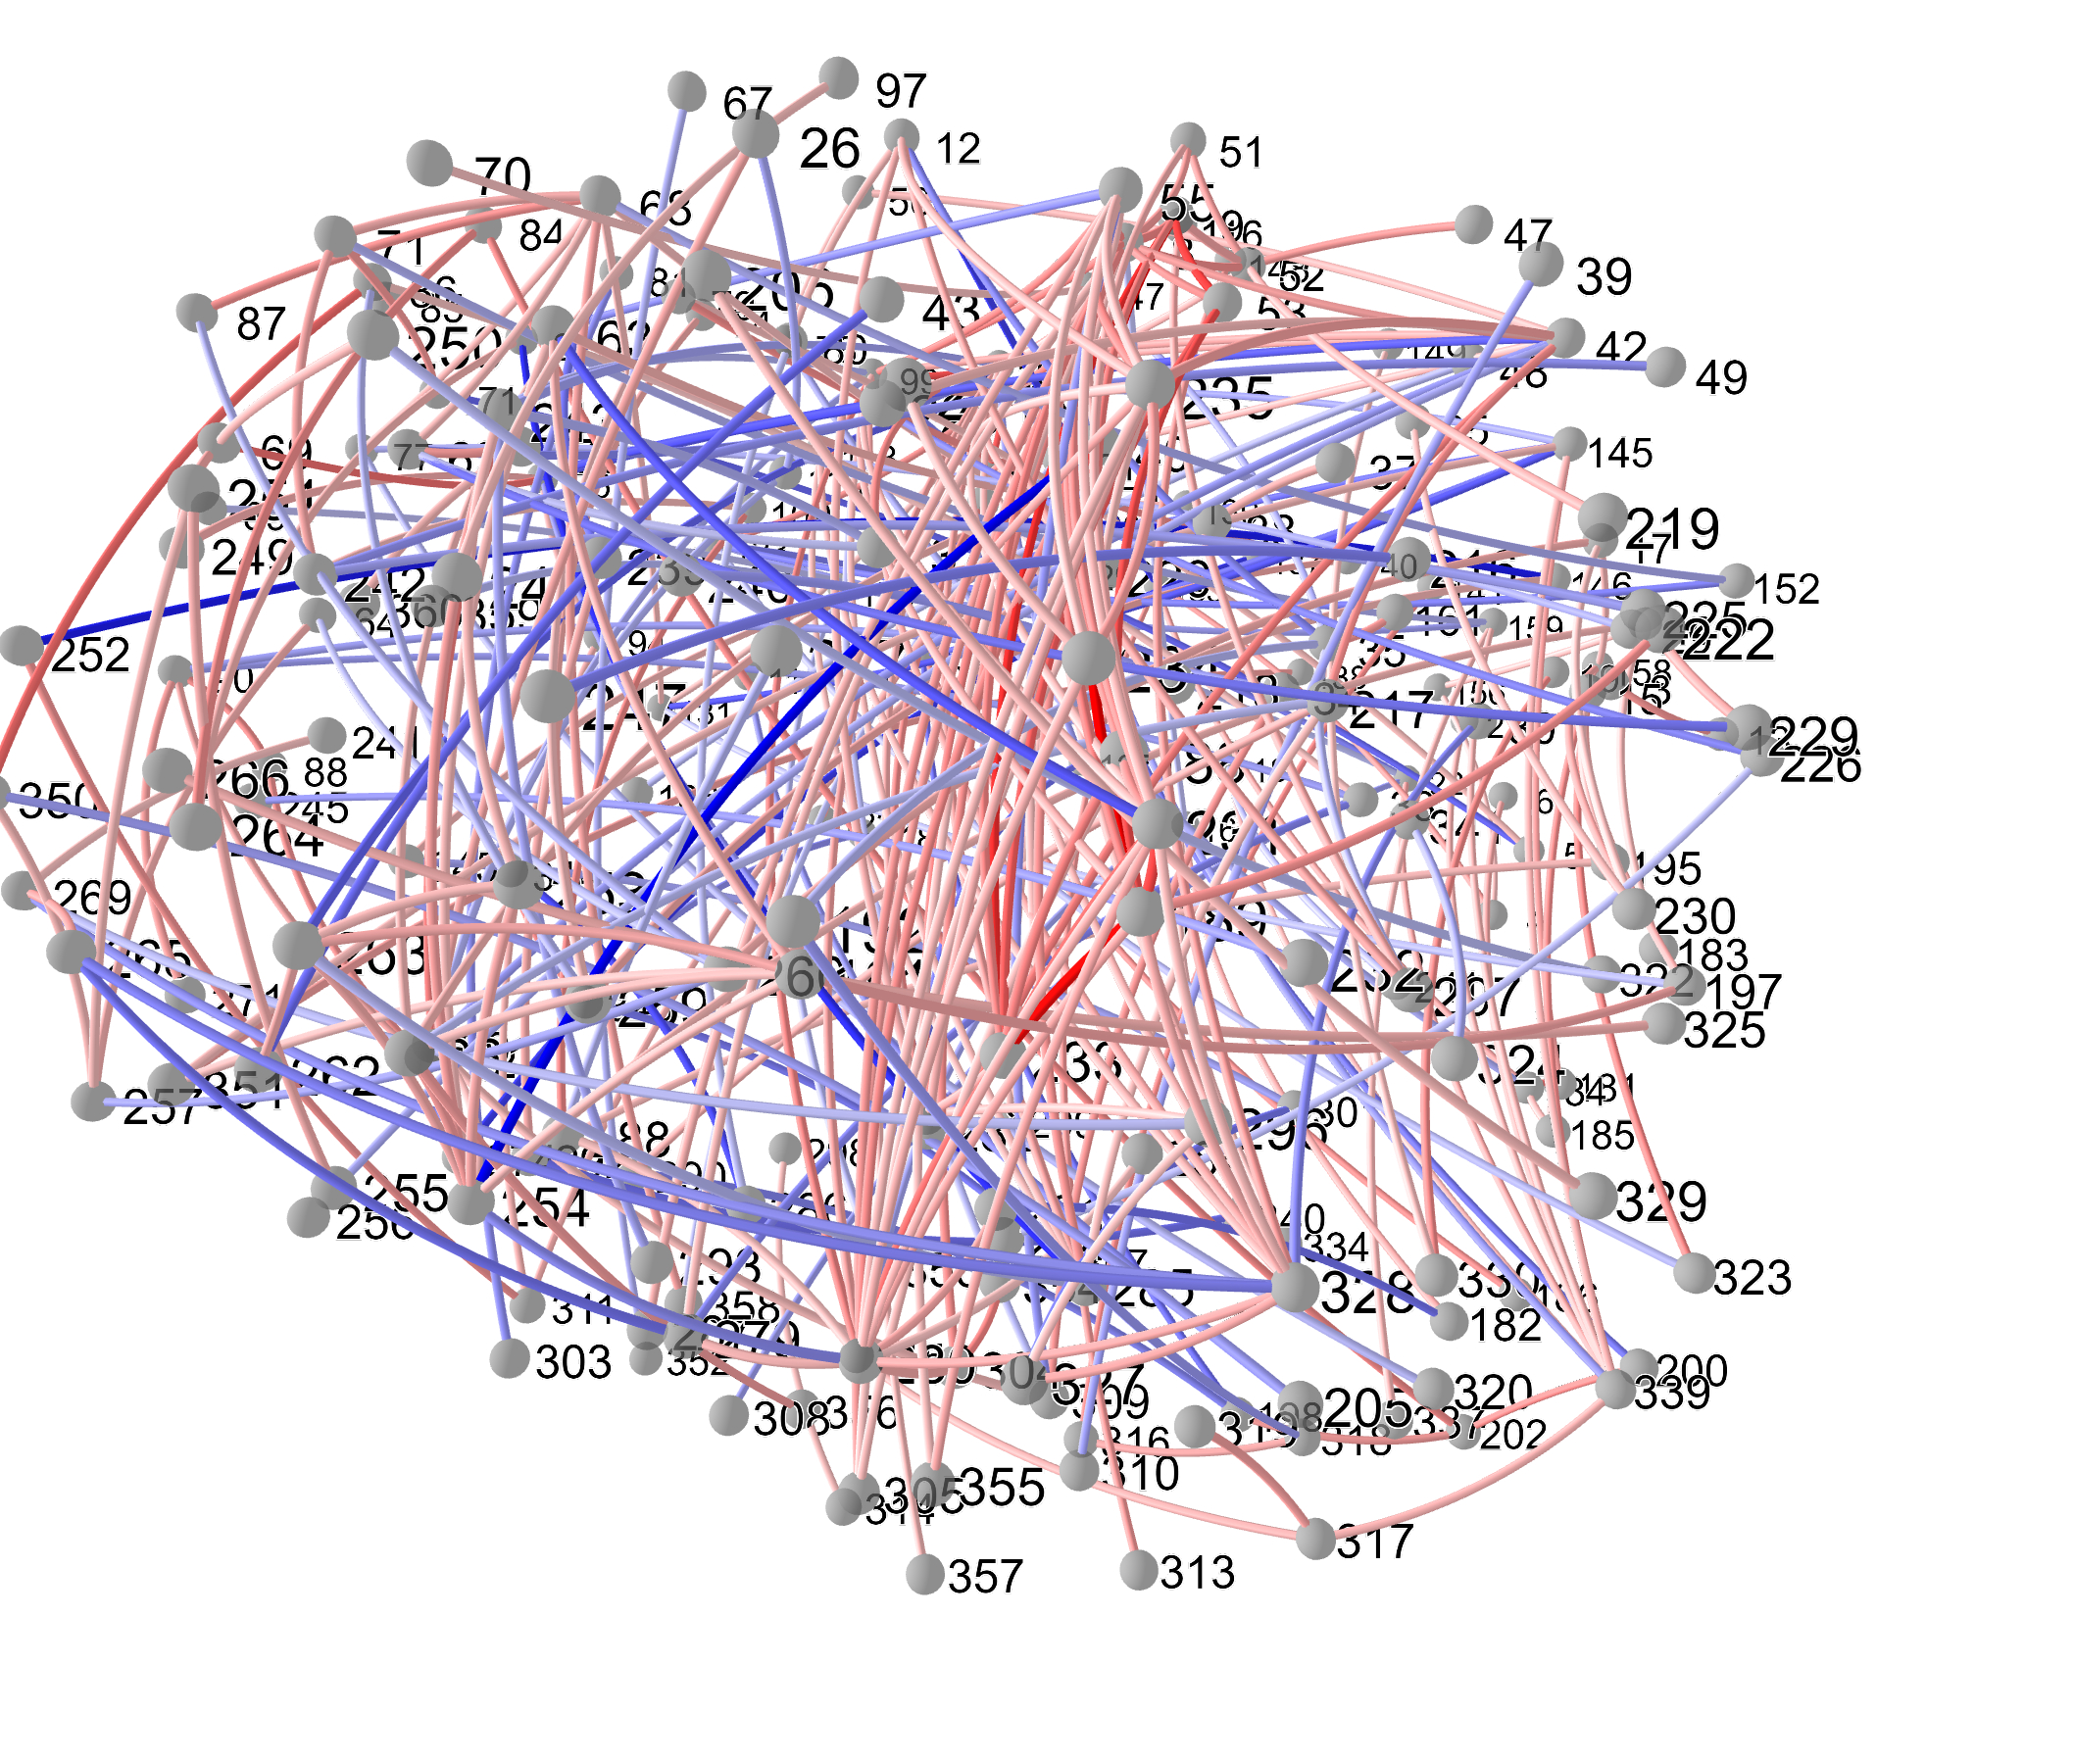
\includegraphics[scale=0.1]{3d_graph.jpg}
\caption{Ejemplo de representación de grafo en tres dimensiones con los nodos distribuídos según la forma del cerebro}
\end{figure}

Usando la opción de \texttt{Many-Body Force} existen distintos tipos de fuerzas e interacciones entre los nodos y las arista,
las cuales se pueden modificar, entre ellas: \texttt{Links Force} la cual es la fuerza que ejercen las aristas sobre los nodos
enlazados, \texttt{Collision Force} que es la fuerza de repulsión entre nodos, \texttt{Centering Force} esta atrae a los nodos hacia el centro de la gráfica, \texttt{x Force} y \texttt{y Force} que son las fuerzas que atraen a los nodos hacia el eje señalado.\\

\begin{figure}[h!]%
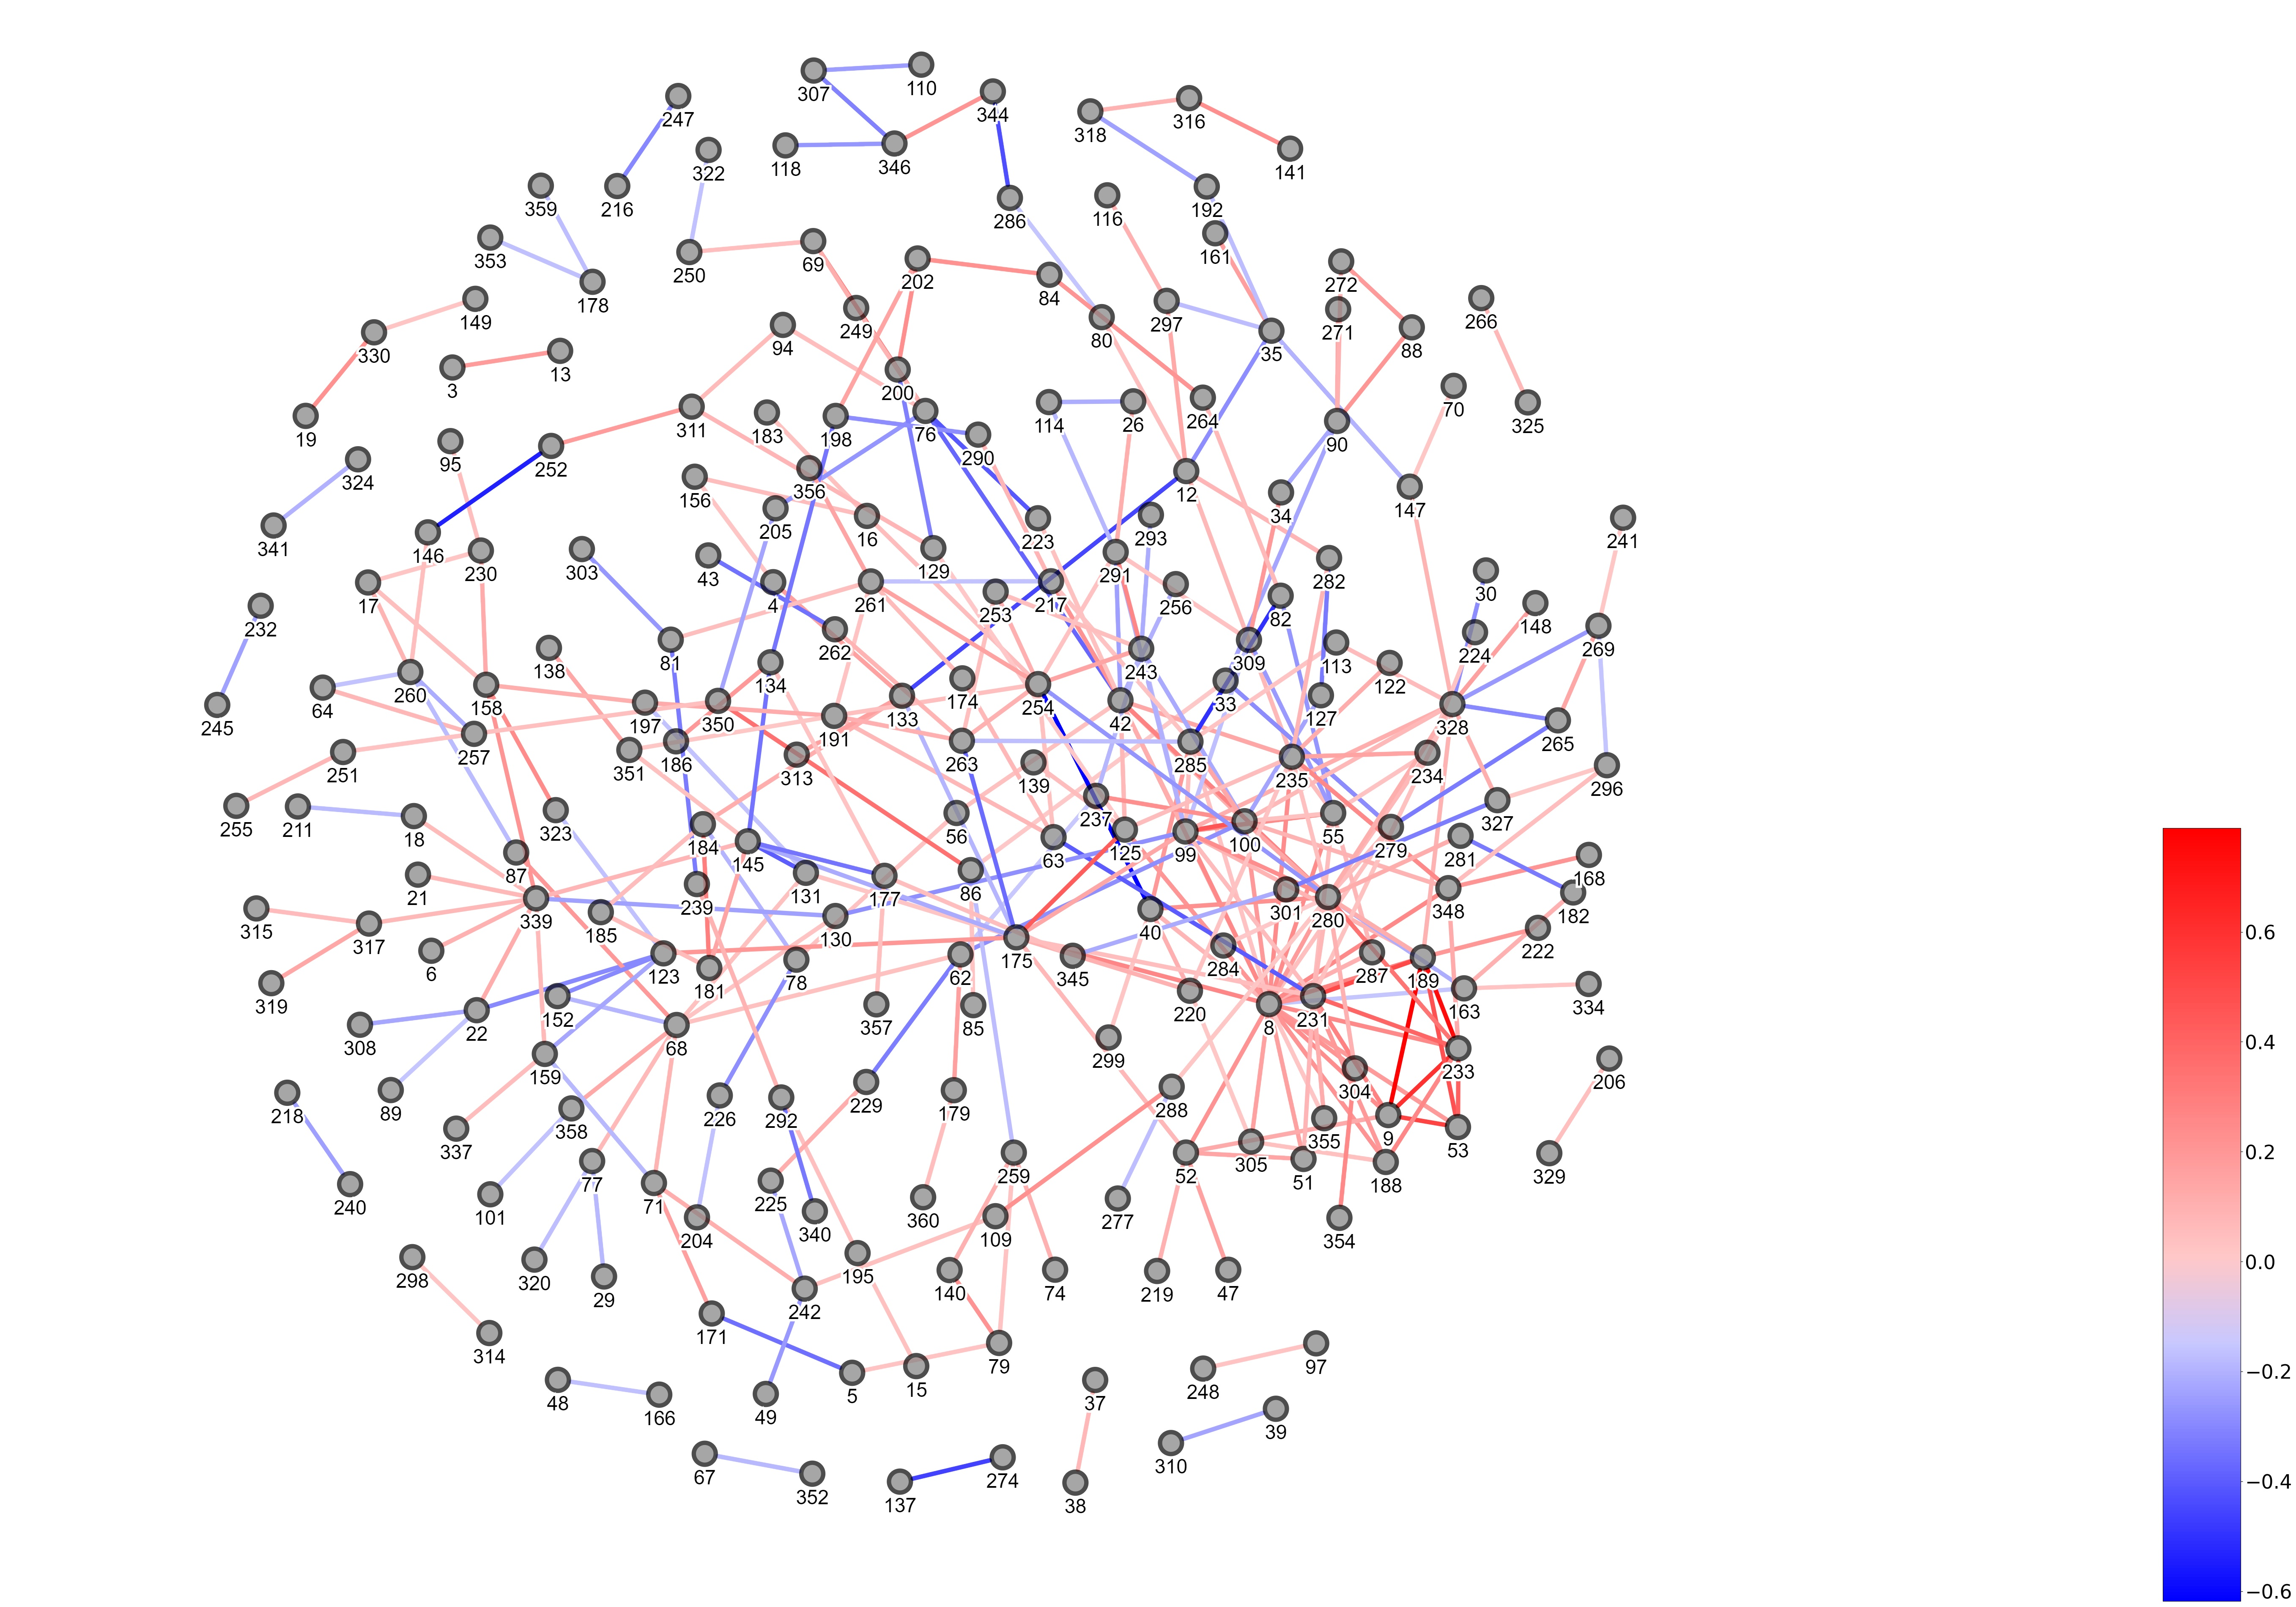
\includegraphics[scale=0.05]{graph_colorbar.jpg}
\caption{Representación de un grafo que representa las conexiones contemporáneas y lass fuerzas de los enlaces con los colores de las aristas}
\end{figure}


\begin{figure}[h!]%
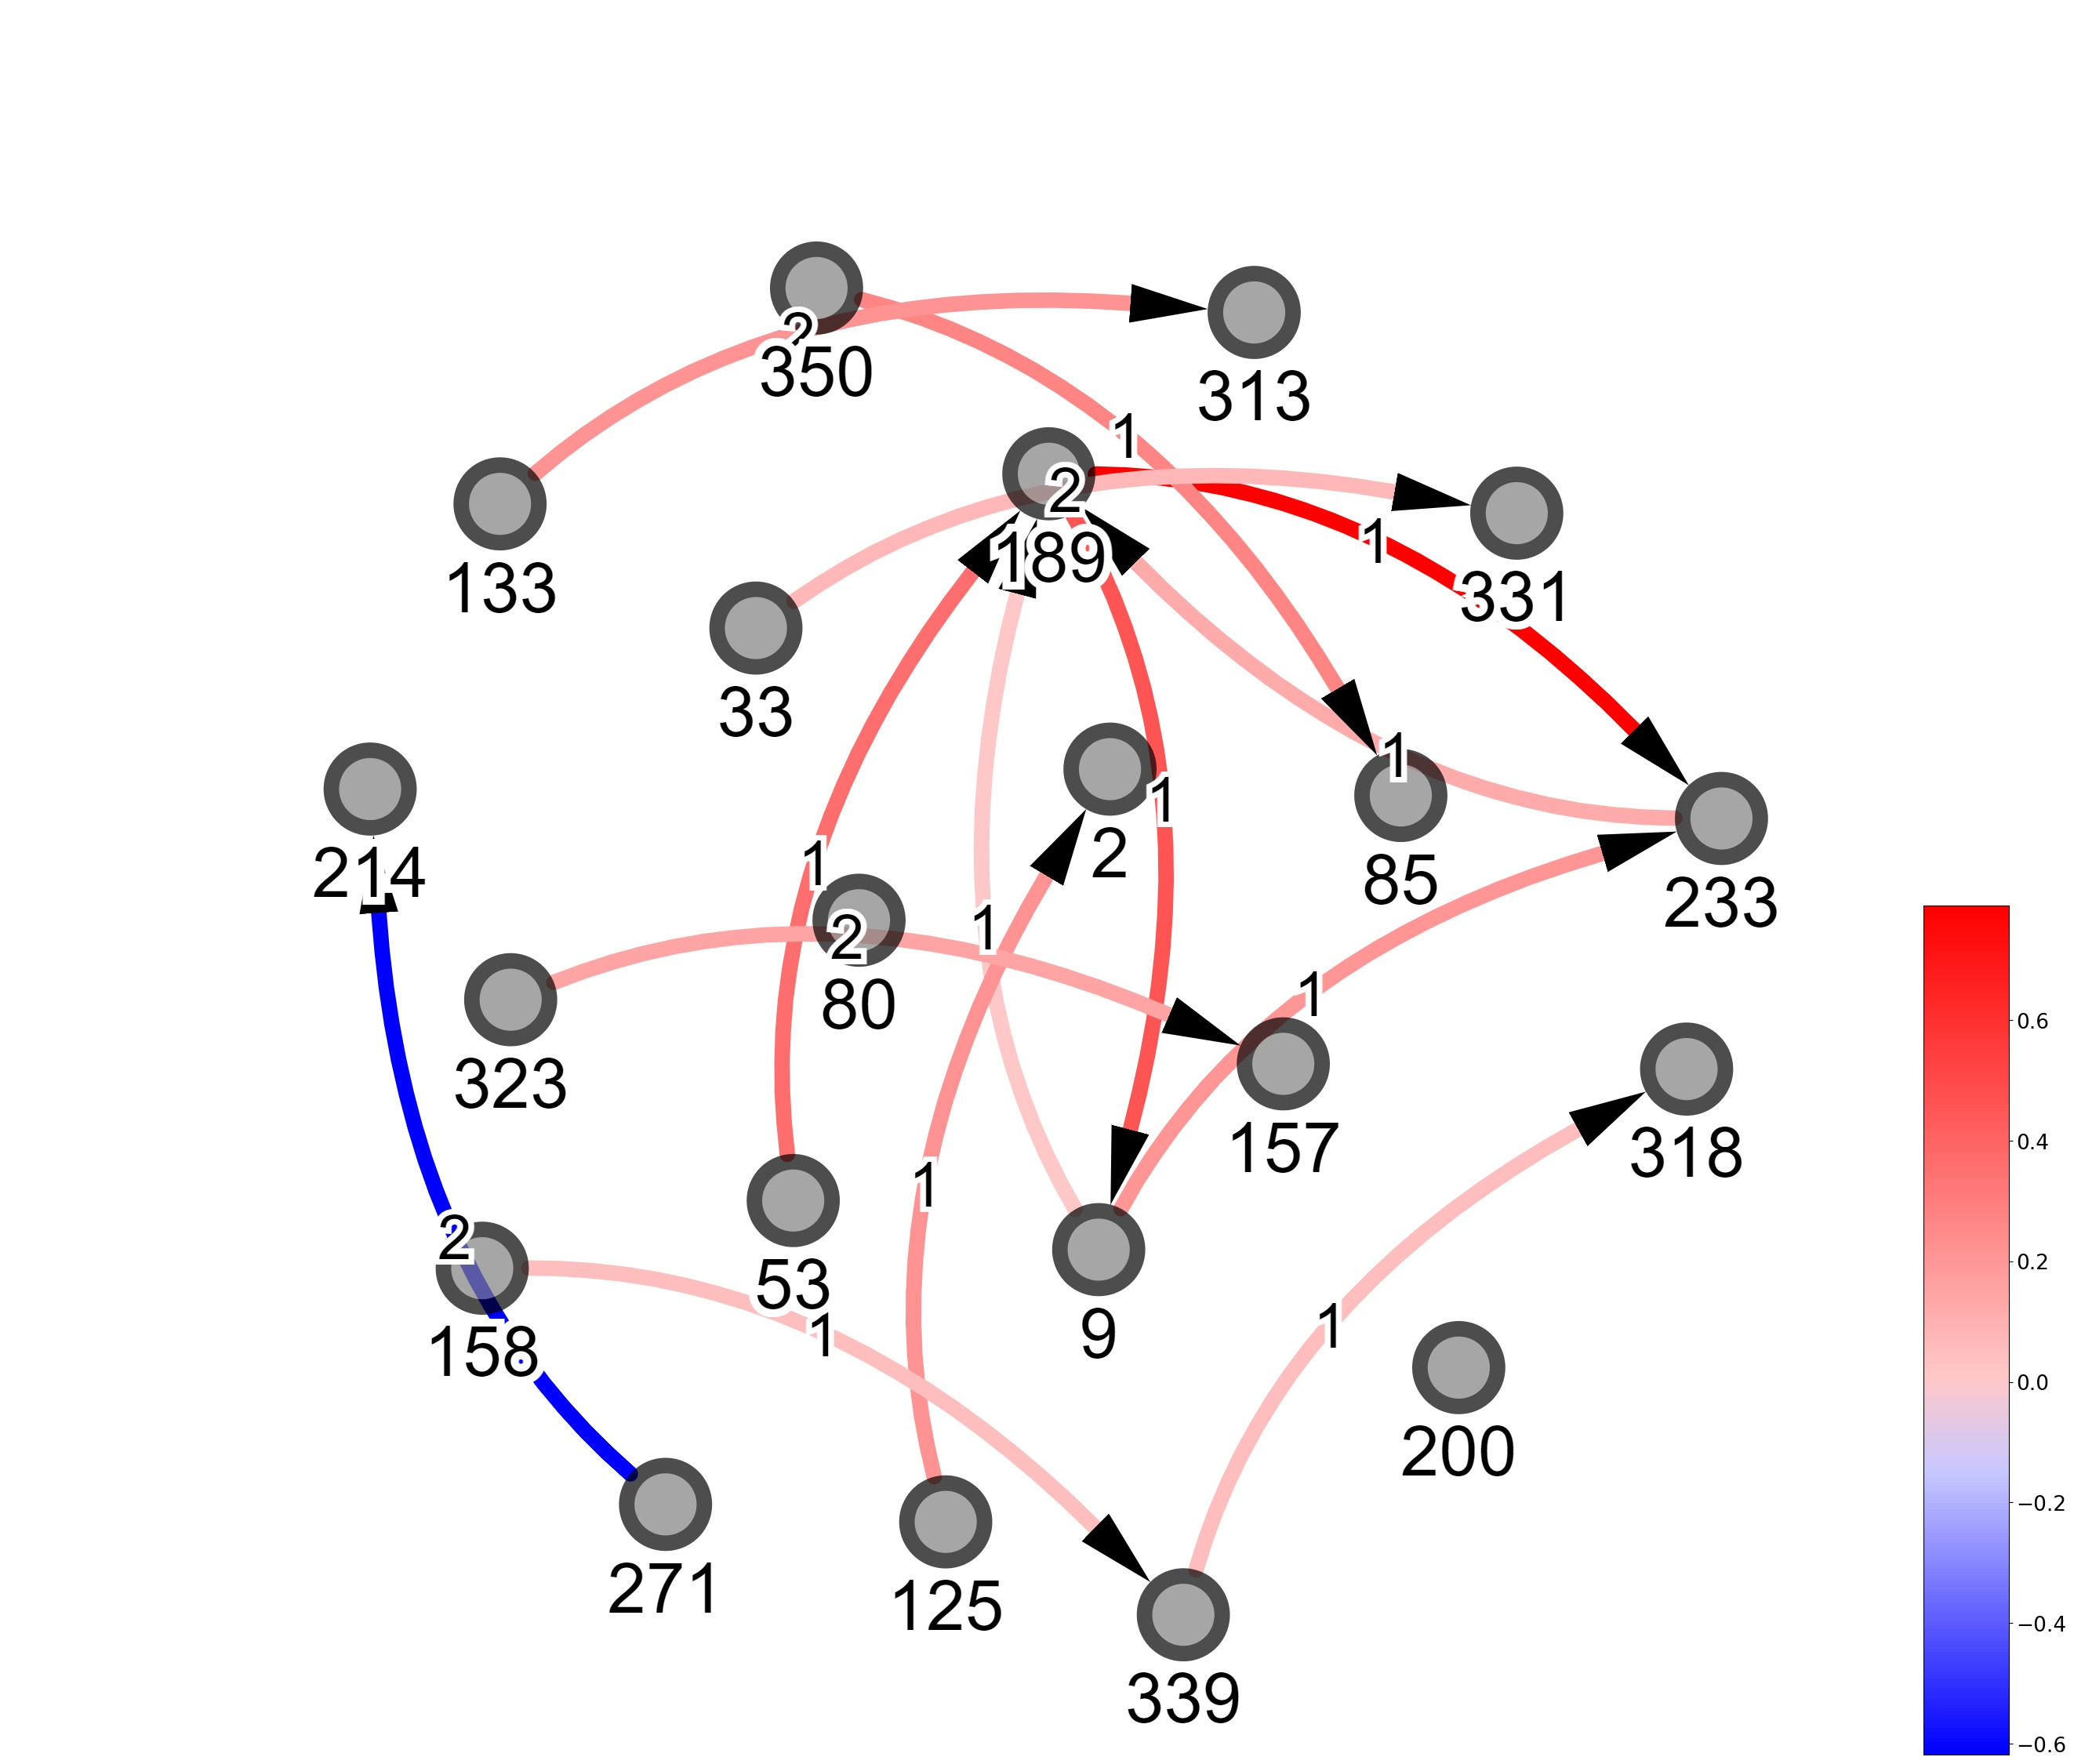
\includegraphics[scale=0.1]{digraph_colorbar.jpg}
\caption{Representación de un grafo dirigido que representa las conexiones causales}
\end{figure}

En el caso de las representaciones de \texttt{Complex Graph} además de estas físicas anteriores, tambien se permiten seleccionar distintos algoritmos para la representación, como es el caso del algoritmo de Barnes-Hut, este divide recursivamente los $n$ cuerpos en grupos almacenándolos en octábolos, mientras que el espacio se subdivide recursivamente en octantes hasta que cada subdivisión tenga $0$ o $1$ cuerpos.\\

\begin{figure}[h!]%
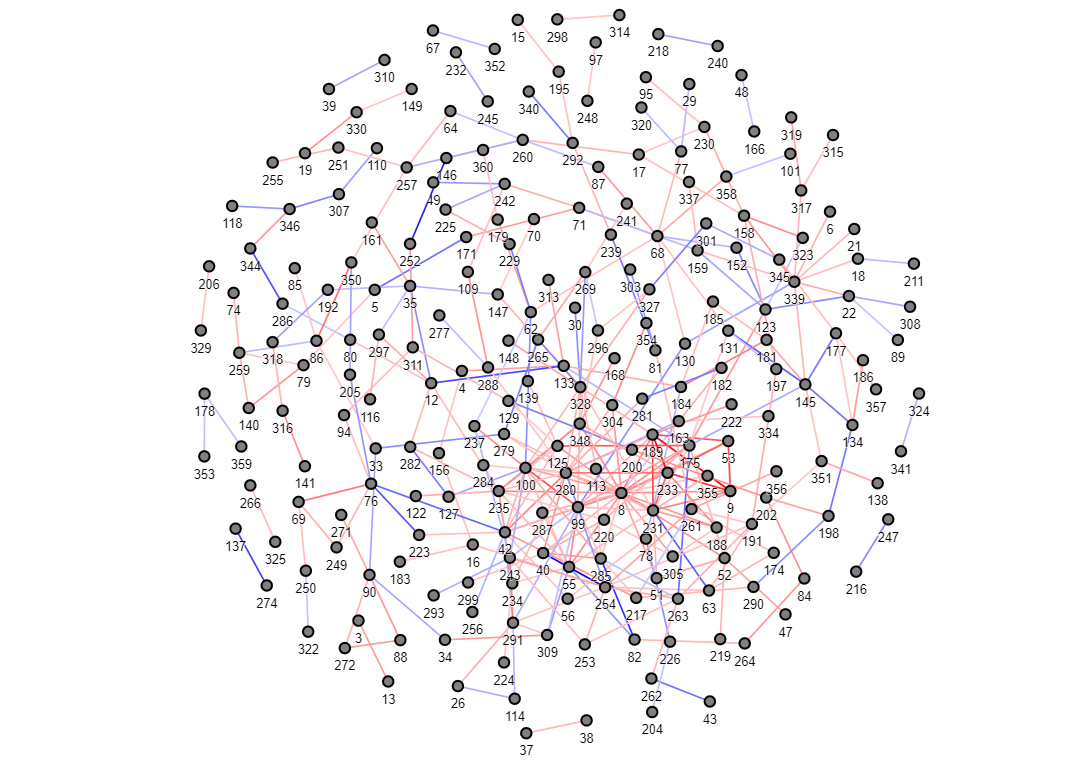
\includegraphics[scale=0.25]{complex.jpg}
\caption{Ejemplo de representación de tipo Complex Graph}
\end{figure}

Aplicando estas representaciones con físicas se logra una graficación más factorizada, logrando facilitar al usuario las visualización
de los resultados, además de logar optimizar en tiempo de ejecución y procesamiento, pues los algoritmos que se usan tienen una complejidad temporal máxima de $O(n\log{n})$.\\

%===================================================================================
% Conclusiones
%-----------------------------------------------------------------------------------
\section{Conclusiones}\label{sec:conc}

  En esta sección puede incluir las conclusiones de su investigación y las ideas
  sobre la continuidad del trabajo, en el caso que aplique.

%===================================================================================



%===================================================================================
% Recomendaciones
%-----------------------------------------------------------------------------------
\section{Recomendaciones}\label{sec:rec}

Para mejorar este proyecto y que resulte aún más útil se recomienda representar en un solo grafo las conexiones contemporáneas y las conexiones causales, lo cual no pudimos llevar a cabo porque esto necesita tener un grafo con aristas dirigidas y no dirigidas al mismo tiempo, lo que nos imposibilitaría explotar las bondades de librerías como gravis \cite{gv} que hizo todo el proceso de distribuir el grafo en el espacio bidimensional. Por lo que esta mejora llevaría un gran trabajo. \\

Igualmente en los gráficos en tres dimensiones, los cuales se organizan para tener forma cerebral, una mejora visual sería que curvear las aristas de forma que simule mejor la forma del cerebro y añadir una imagen del cerebro debajo para que se vea realmente que zona de este representa cada nodo.

%===================================================================================



%===================================================================================
% Bibliografía
%-----------------------------------------------------------------------------------
\begin{thebibliography}{99}
%-----------------------------------------------------------------------------------
	%\bibitem{knuth} Donald E. Knuth. \emph{The Art of Computer Programming}.
%		Volume 1: Fundamental Algorithms (3rd~edition), 1997.
	%	Addison-Wesley Professional.

	\bibitem{gv}Documentación de la librería de python gravis \href{https://robert-haas.github.io/gravis-docs/}{https://robert-haas.github.io/gravis-docs}.

	\bibitem{st}Documentación de la librería de python streamlit \href{https://docs.streamlit.io}{https://docs.streamlit.io}.



%-----------------------------------------------------------------------------------
\end{thebibliography}

%-----------------------------------------------------------------------------------


\label{end}

\end{document}

%===================================================================================
